\chapter{Задача слежения для системы с астатизмом первого порядка
(И-регулятор)}
Рассмотрим замкнутую систему с интегральным регулятором (Схема задана на рисунке
\hyperref[fig:sim4]{\ref{fig:sim4}}). Зададимся следующими параметрами $k_i$:
\begin{enumerate}
    \item $k_i = 0.1$
    \item $k_i = 0.25$ 
    \item $k_i = 1$
\end{enumerate}
\section{Стационарный режим $g(t) = A$}
Выполним моделирование:
\begin{figure}[H]
    \centering
    \begin{minipage}{0.45\textwidth}
        \centering
        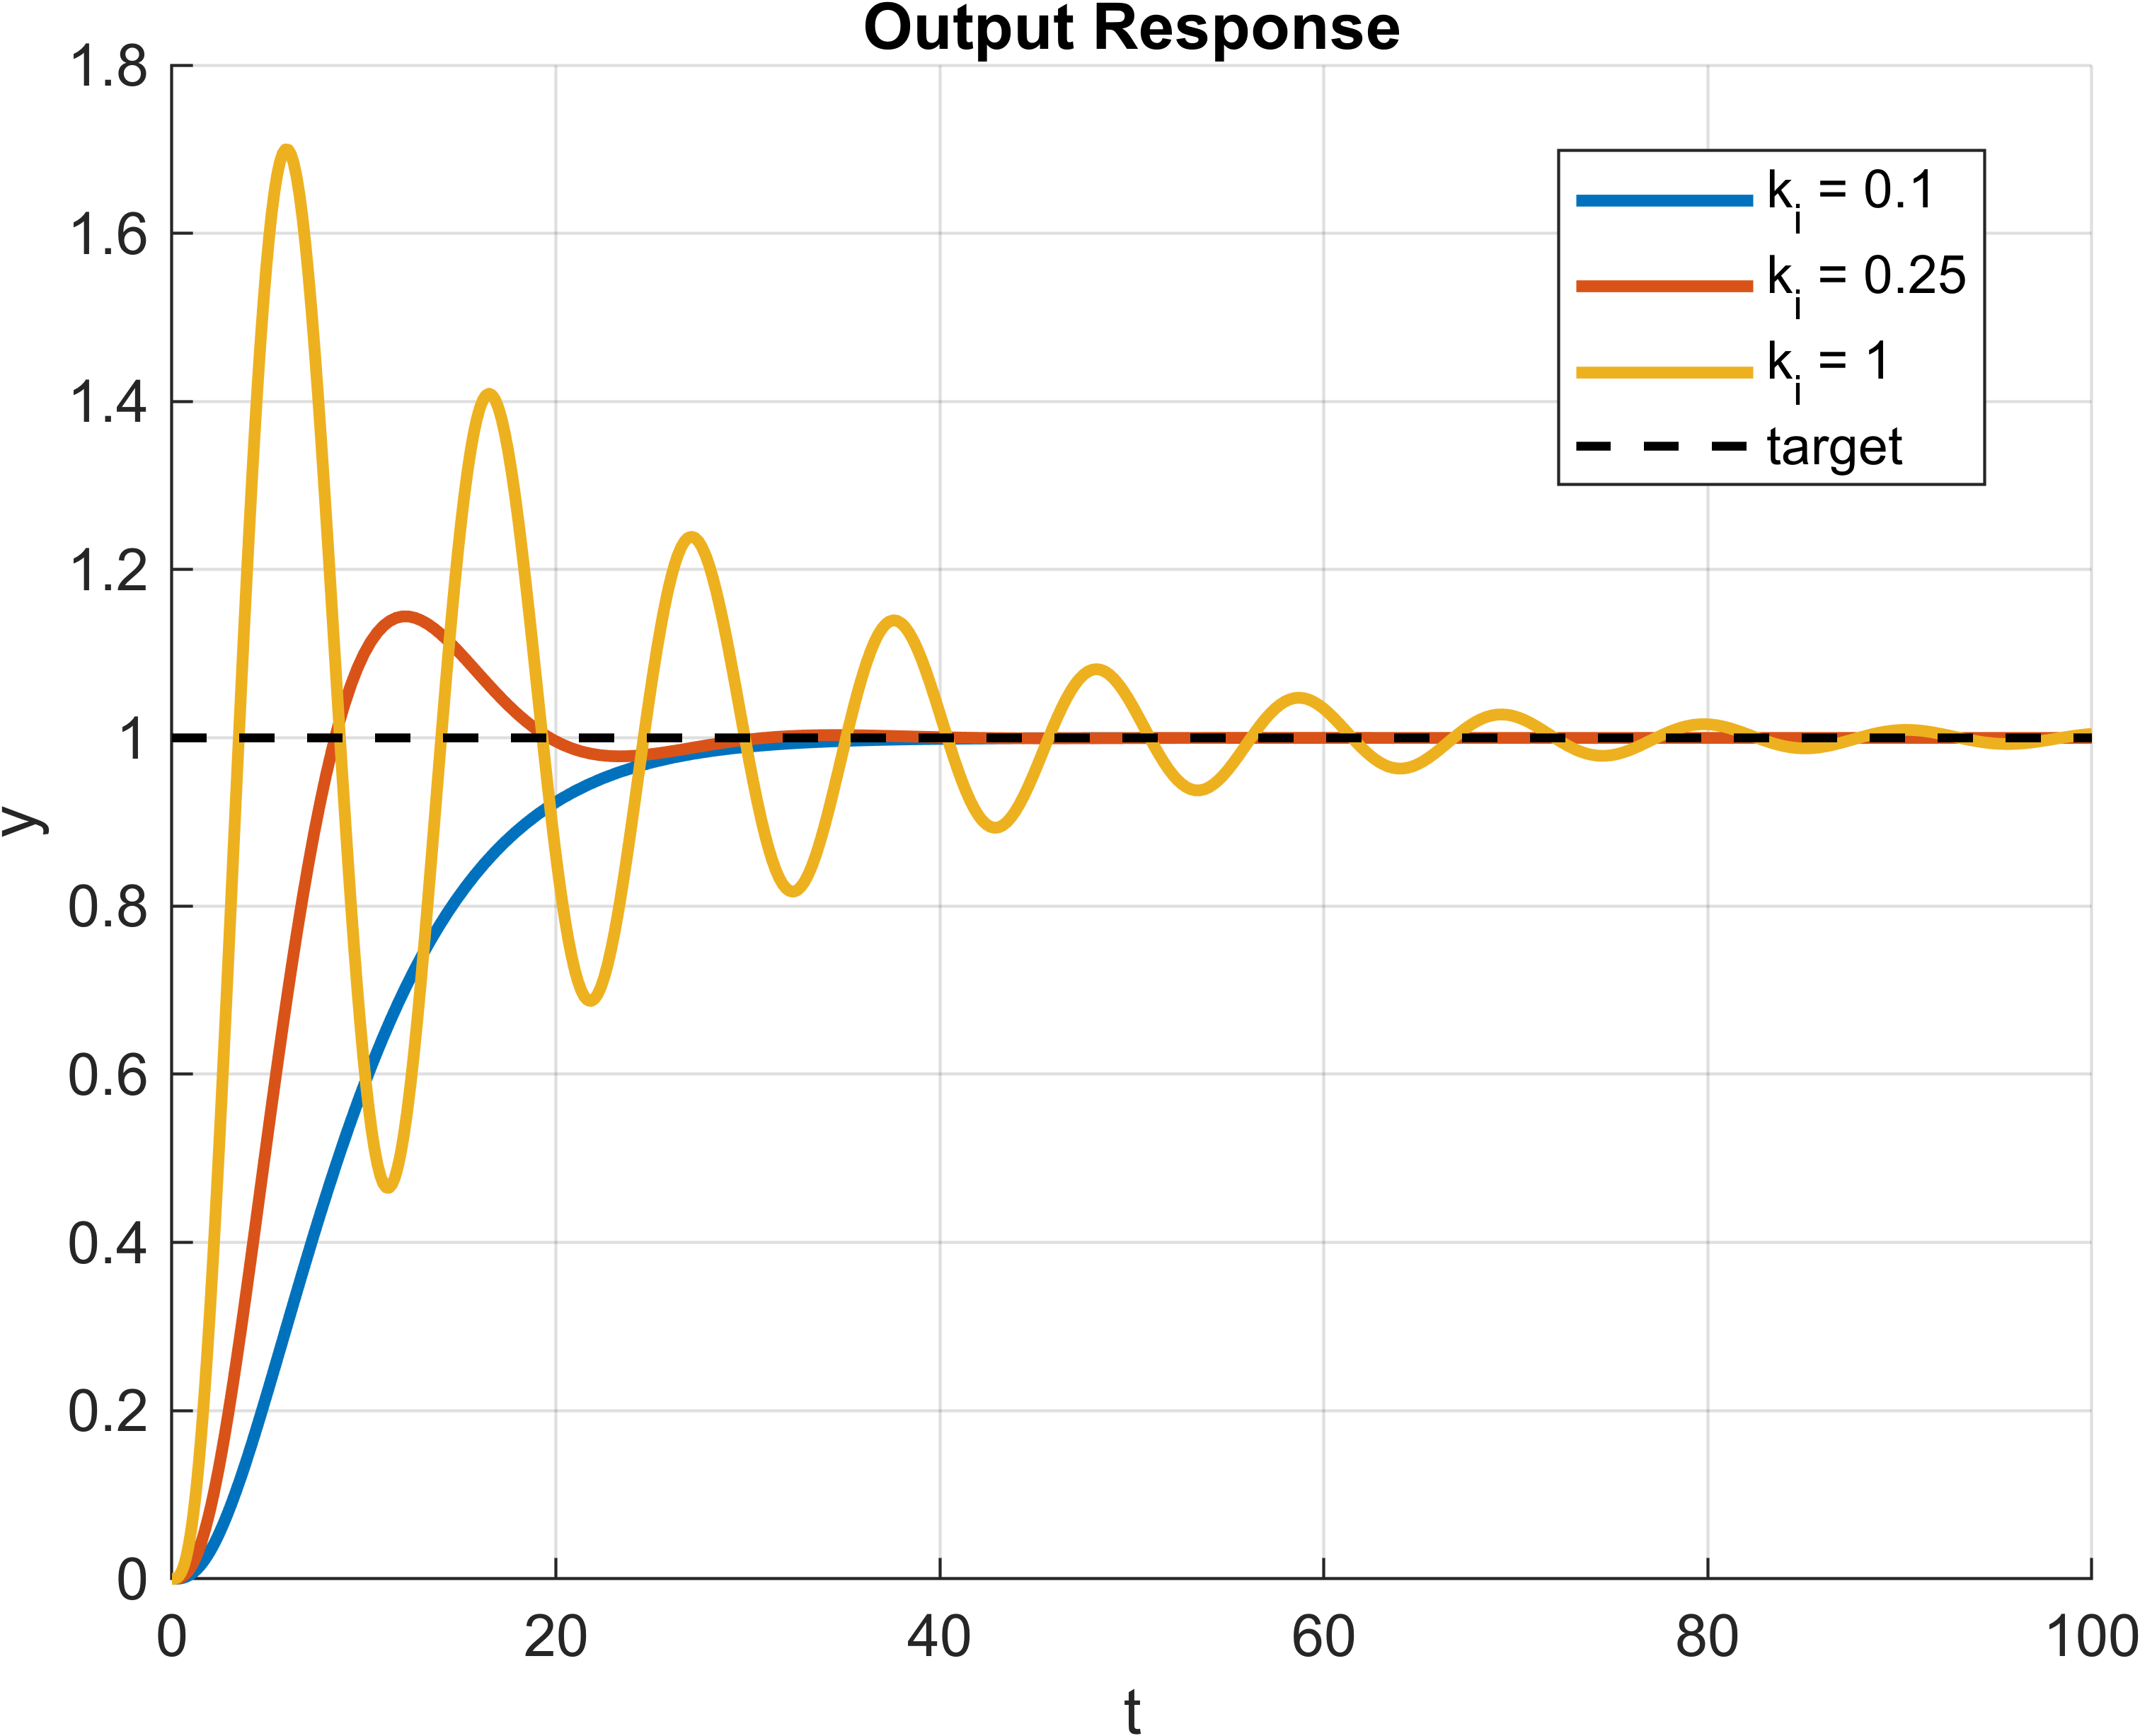
\includegraphics[width=1\textwidth, trim={1cm 0cm 1cm 0cm}]{../images/4_1.png}
    \end{minipage}
    \hfill
    \begin{minipage}{0.45\textwidth}
        \centering
        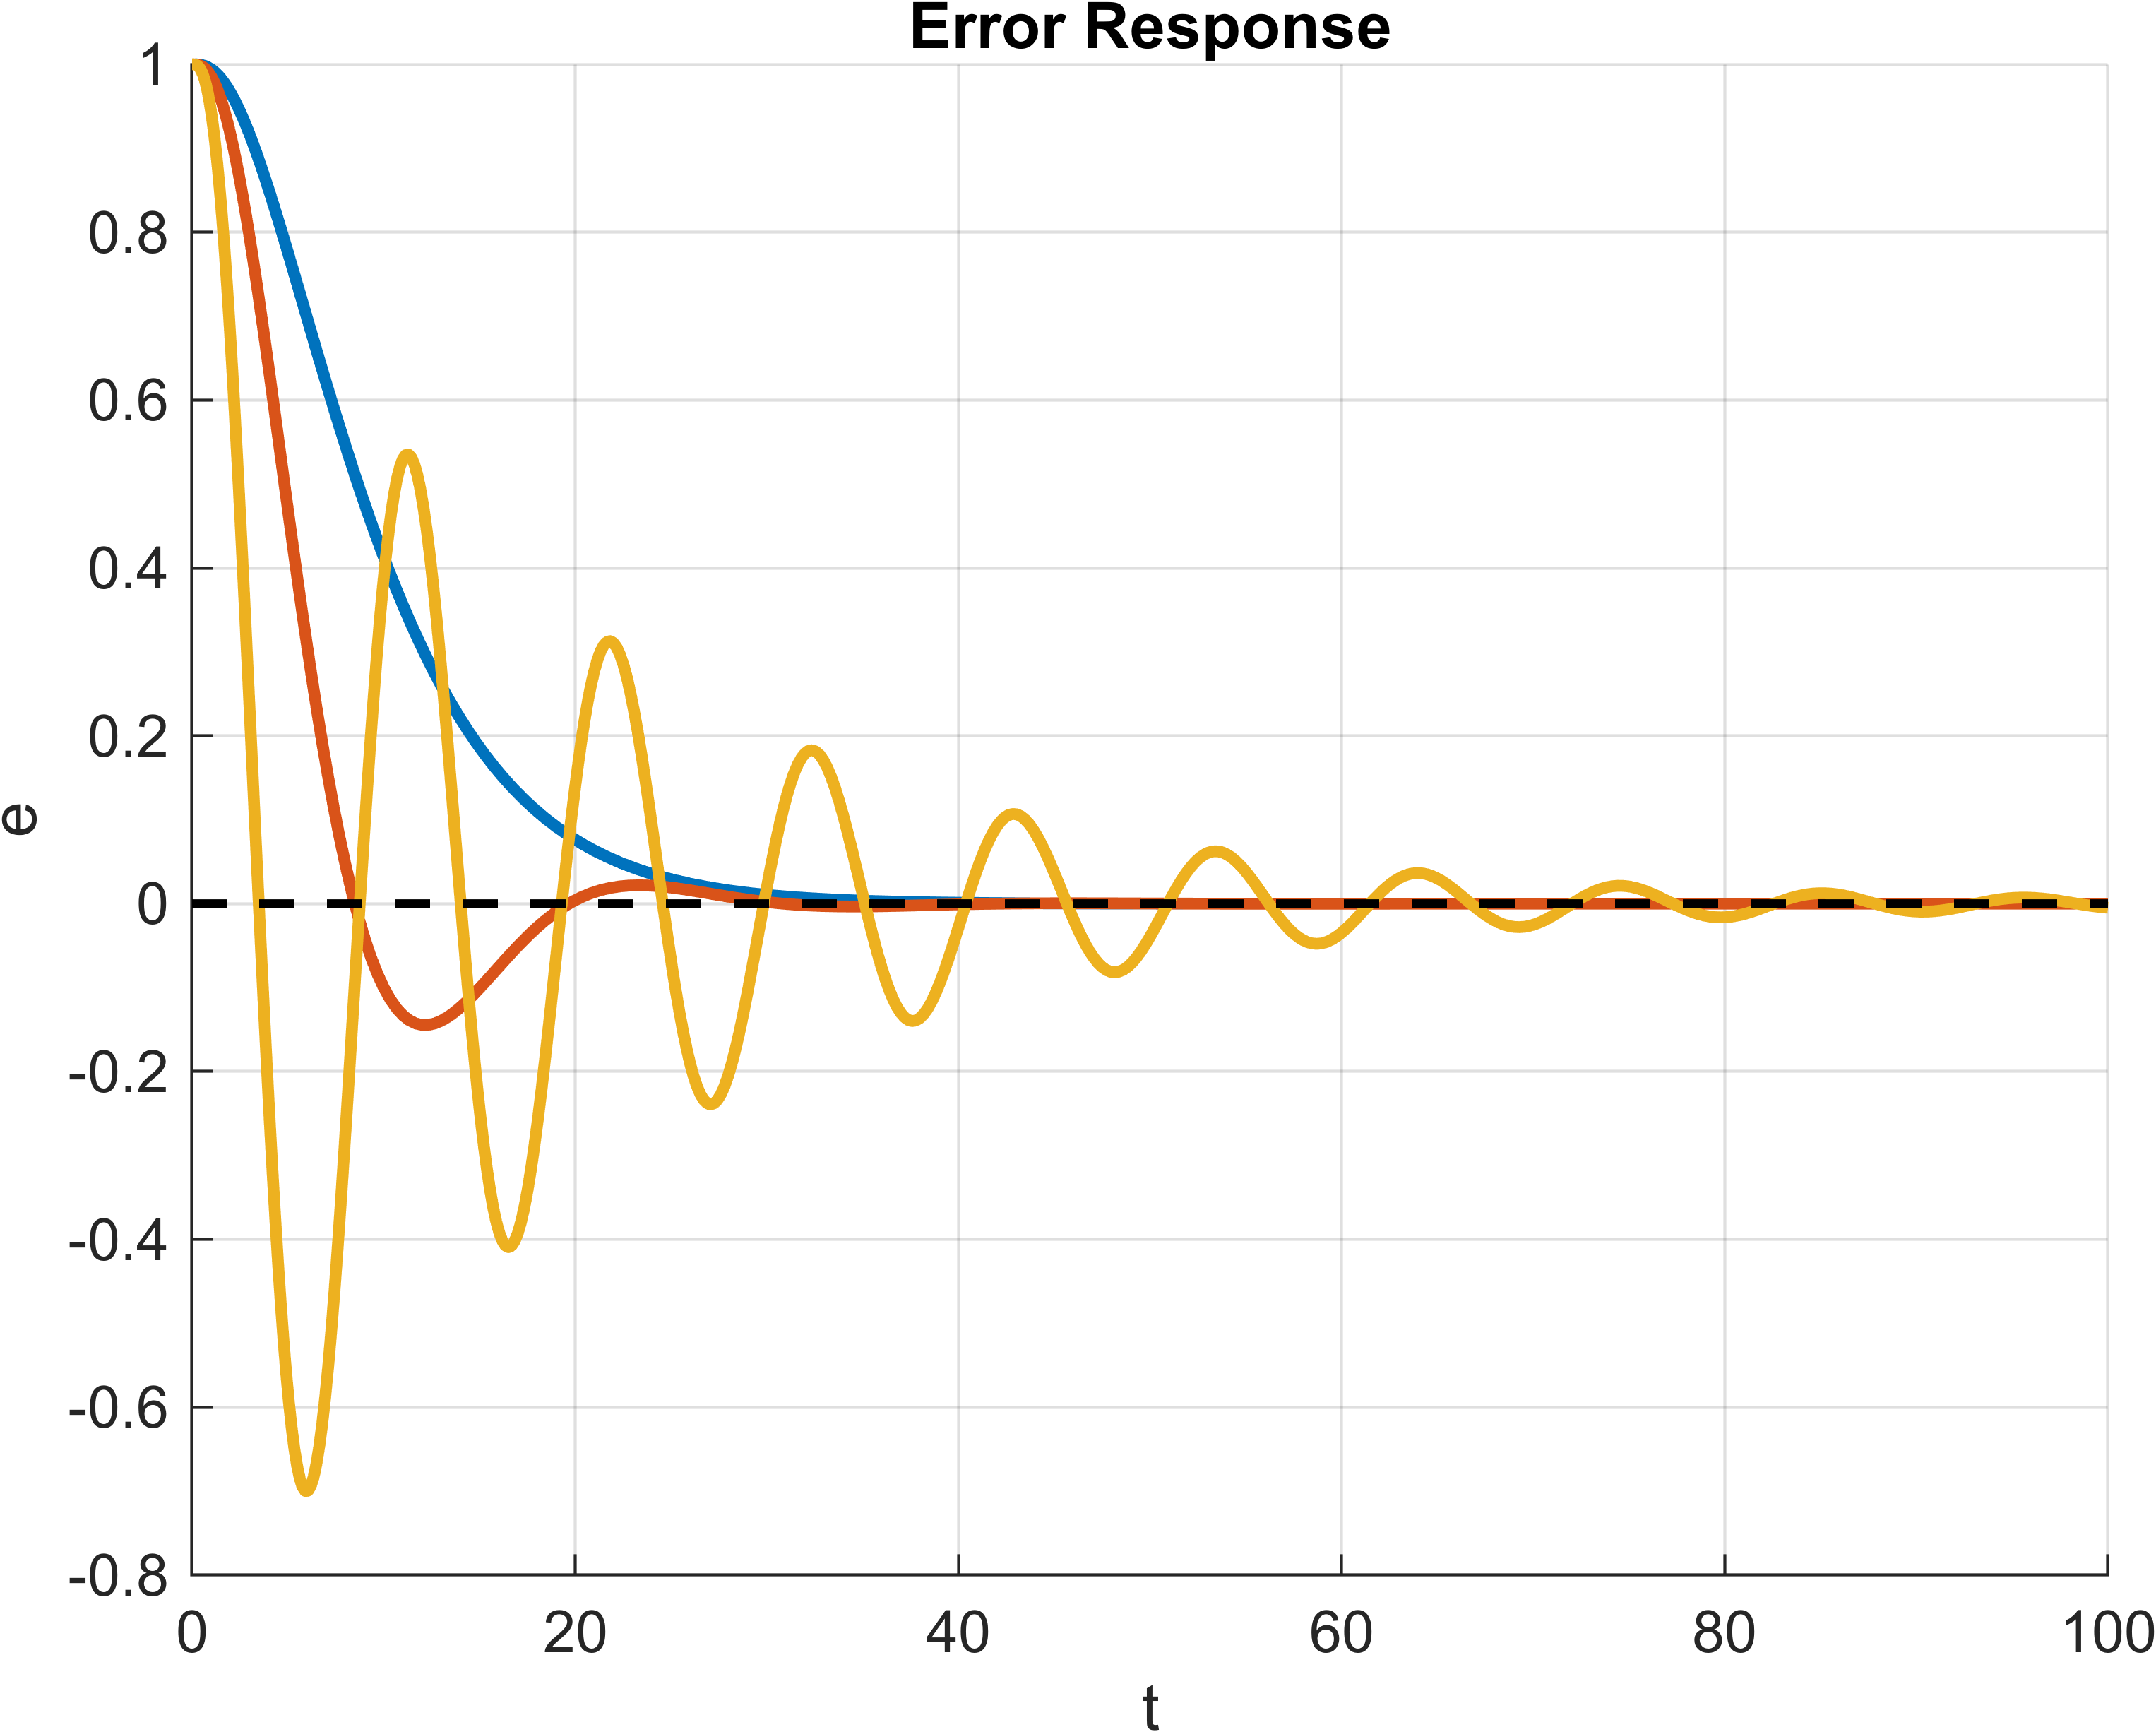
\includegraphics[width=1\textwidth, trim={1cm 0cm 1cm 0cm}]{../images/4_2.png}
    \end{minipage}
    \caption{Графики $y(t)$ и $e(t)$ при $g(t) = 1$}
\end{figure}

Аналитически определим предельное значение ошибки $e$ для каждого значения $k_i$:
\[
W_{g\to e} = \frac{1}{1 + \frac{k_i}{s} W(s)}
= \frac{s}{s + k_i \frac{1}{2s^2 + 3s + 1}}
= \frac{2s^3 + 3s^2 + s}{2s^3 + 3s^2 + s + k_i}
\]
\[
e_{\text{уст}} = \lim_{t \to \infty} e(t)
= \lim_{s \to 0} s E(s)
= \lim_{s \to 0} s W_{g\to e} G(s) =
\]\[
= \lim_{s \to 0} s \frac{2s^3 + 3s^2 + s}{2s^3 + 3s^2 + s + k_i} \frac{1}{s}
= 0
\]

Как видно из графиков и аналитических расчетов, для стационарного режима
И-регулятор обеспечивает нулевую установившуюся ошибку.
\newpage
\section{Режим движения с постоянной скоростью $g(t) = Vt$}
Выполним моделирование:
\begin{figure}[H]
    \centering
    \begin{minipage}{0.45\textwidth}
        \centering
        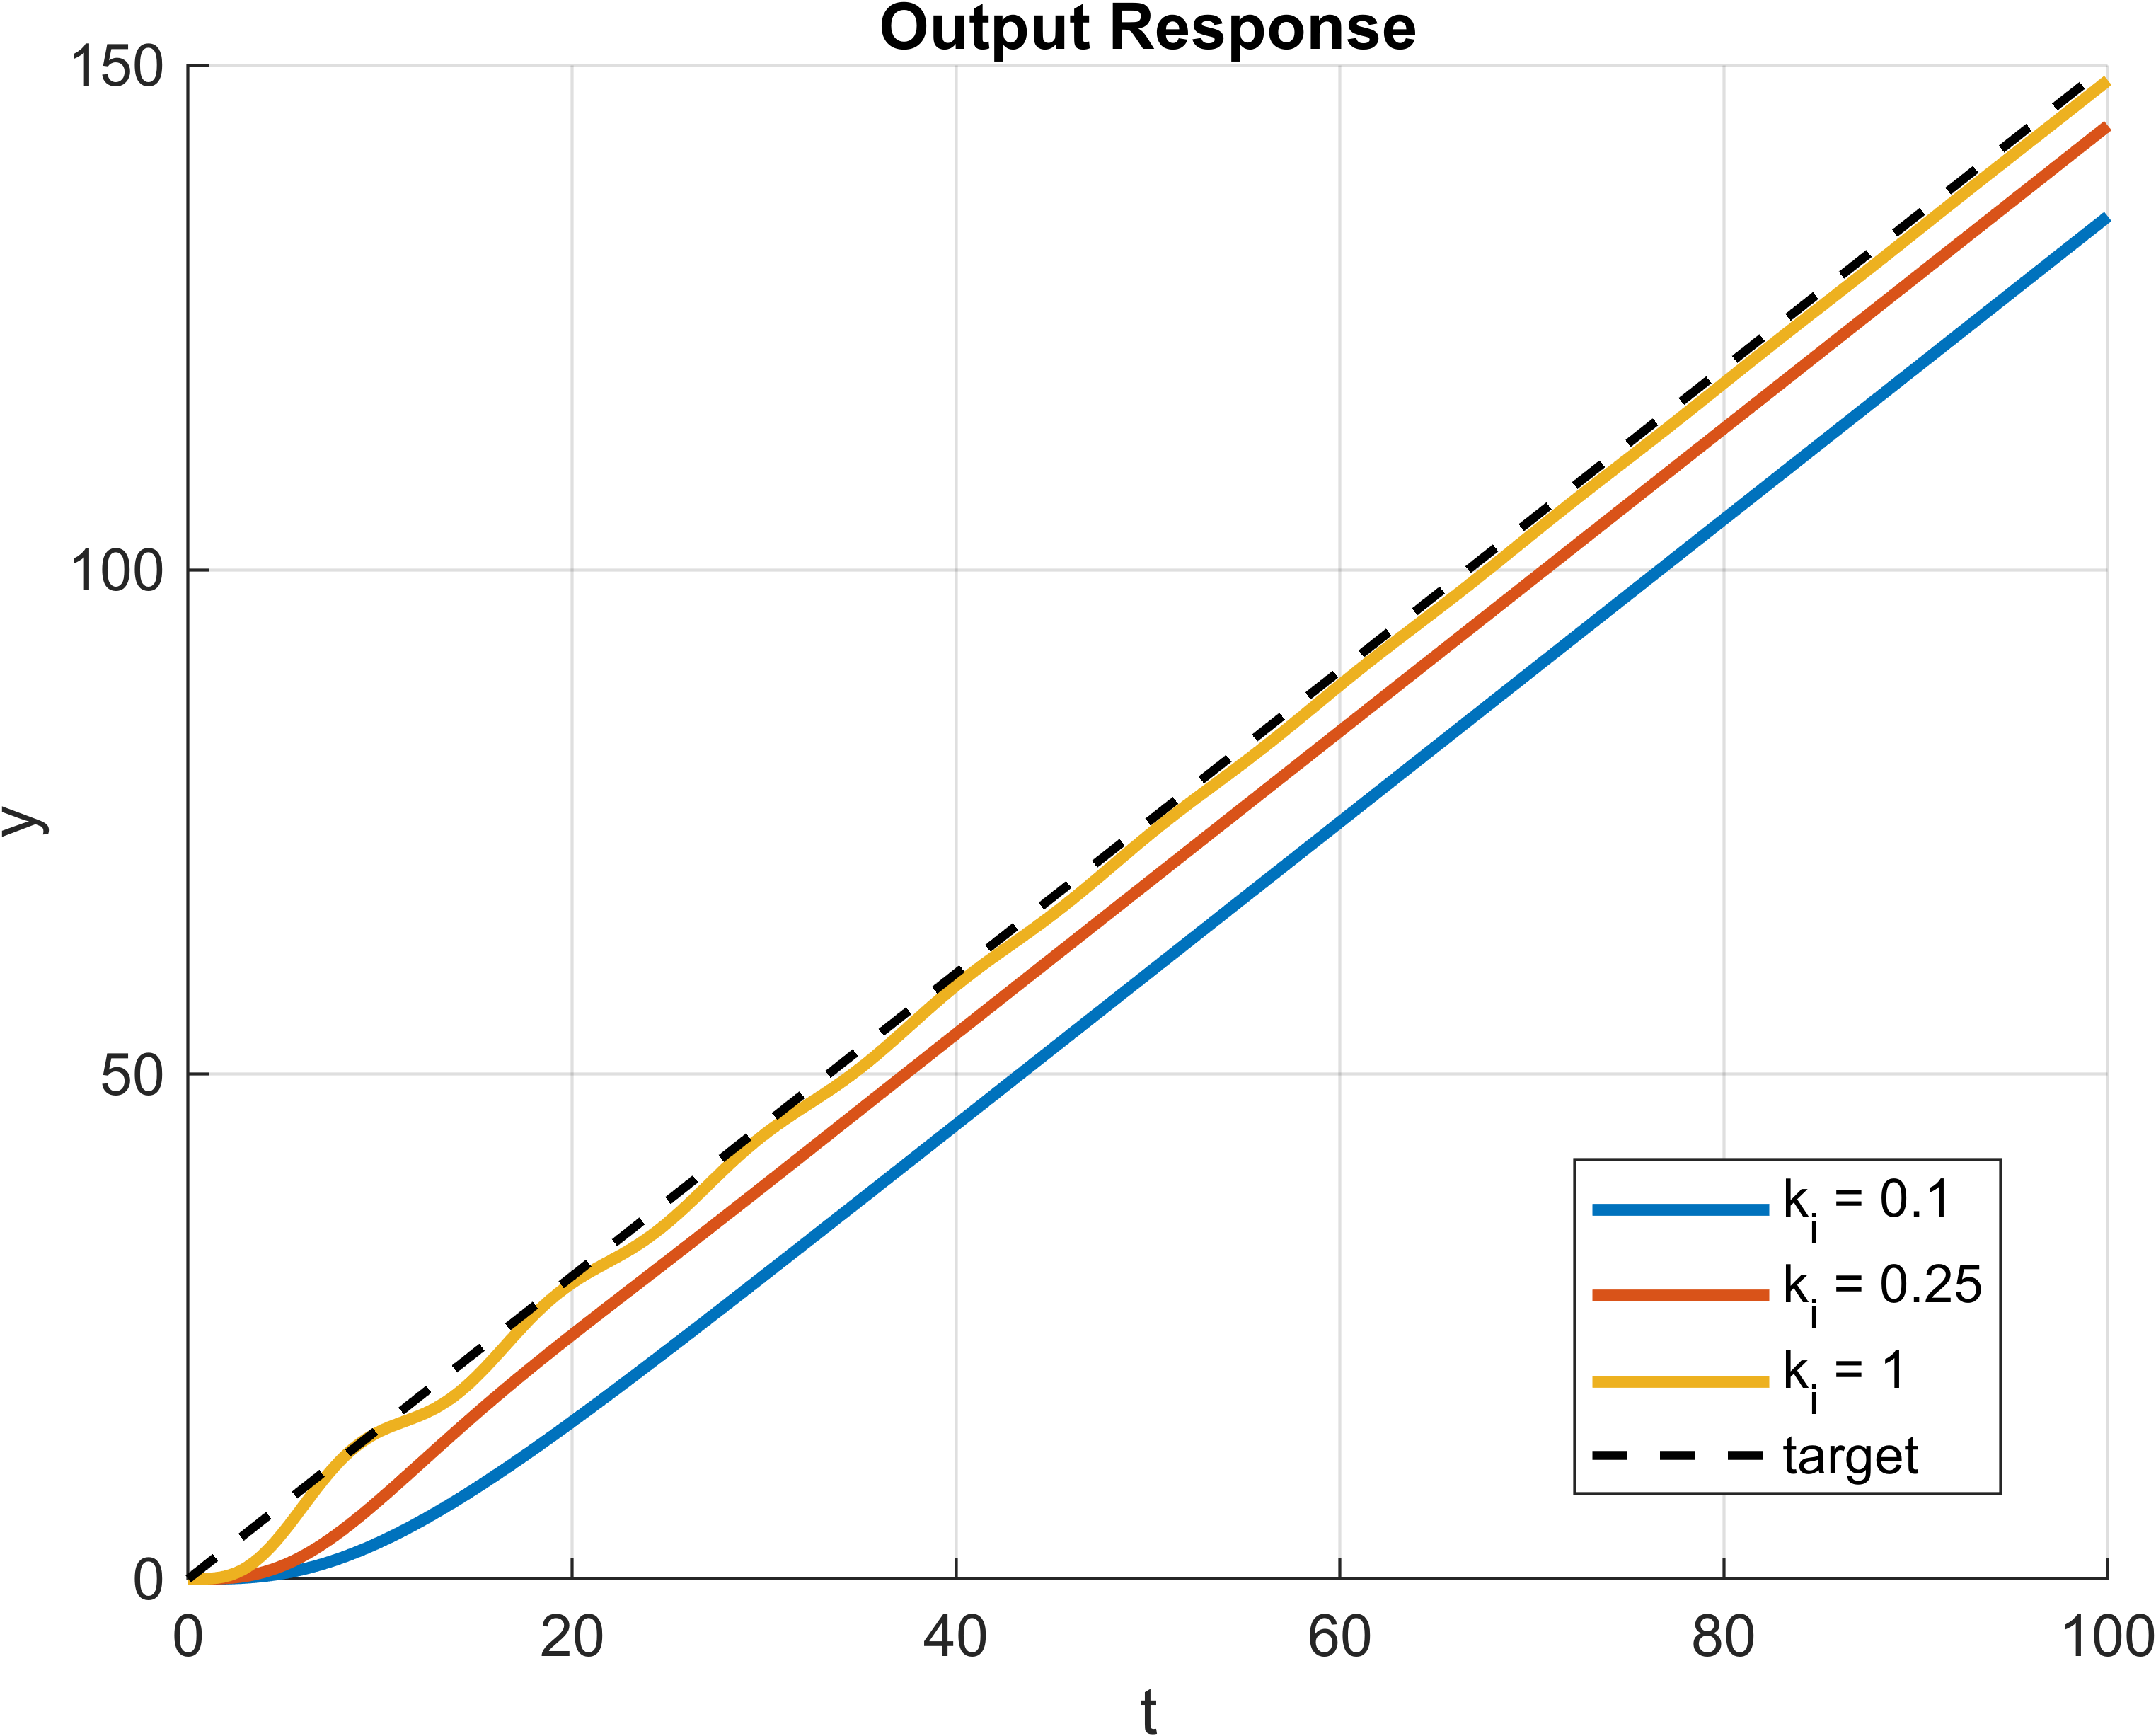
\includegraphics[width=1\textwidth, trim={1cm 0cm 1cm 0cm}]{../images/4_3.png}
    \end{minipage}
    \hfill
    \begin{minipage}{0.45\textwidth}
        \centering
        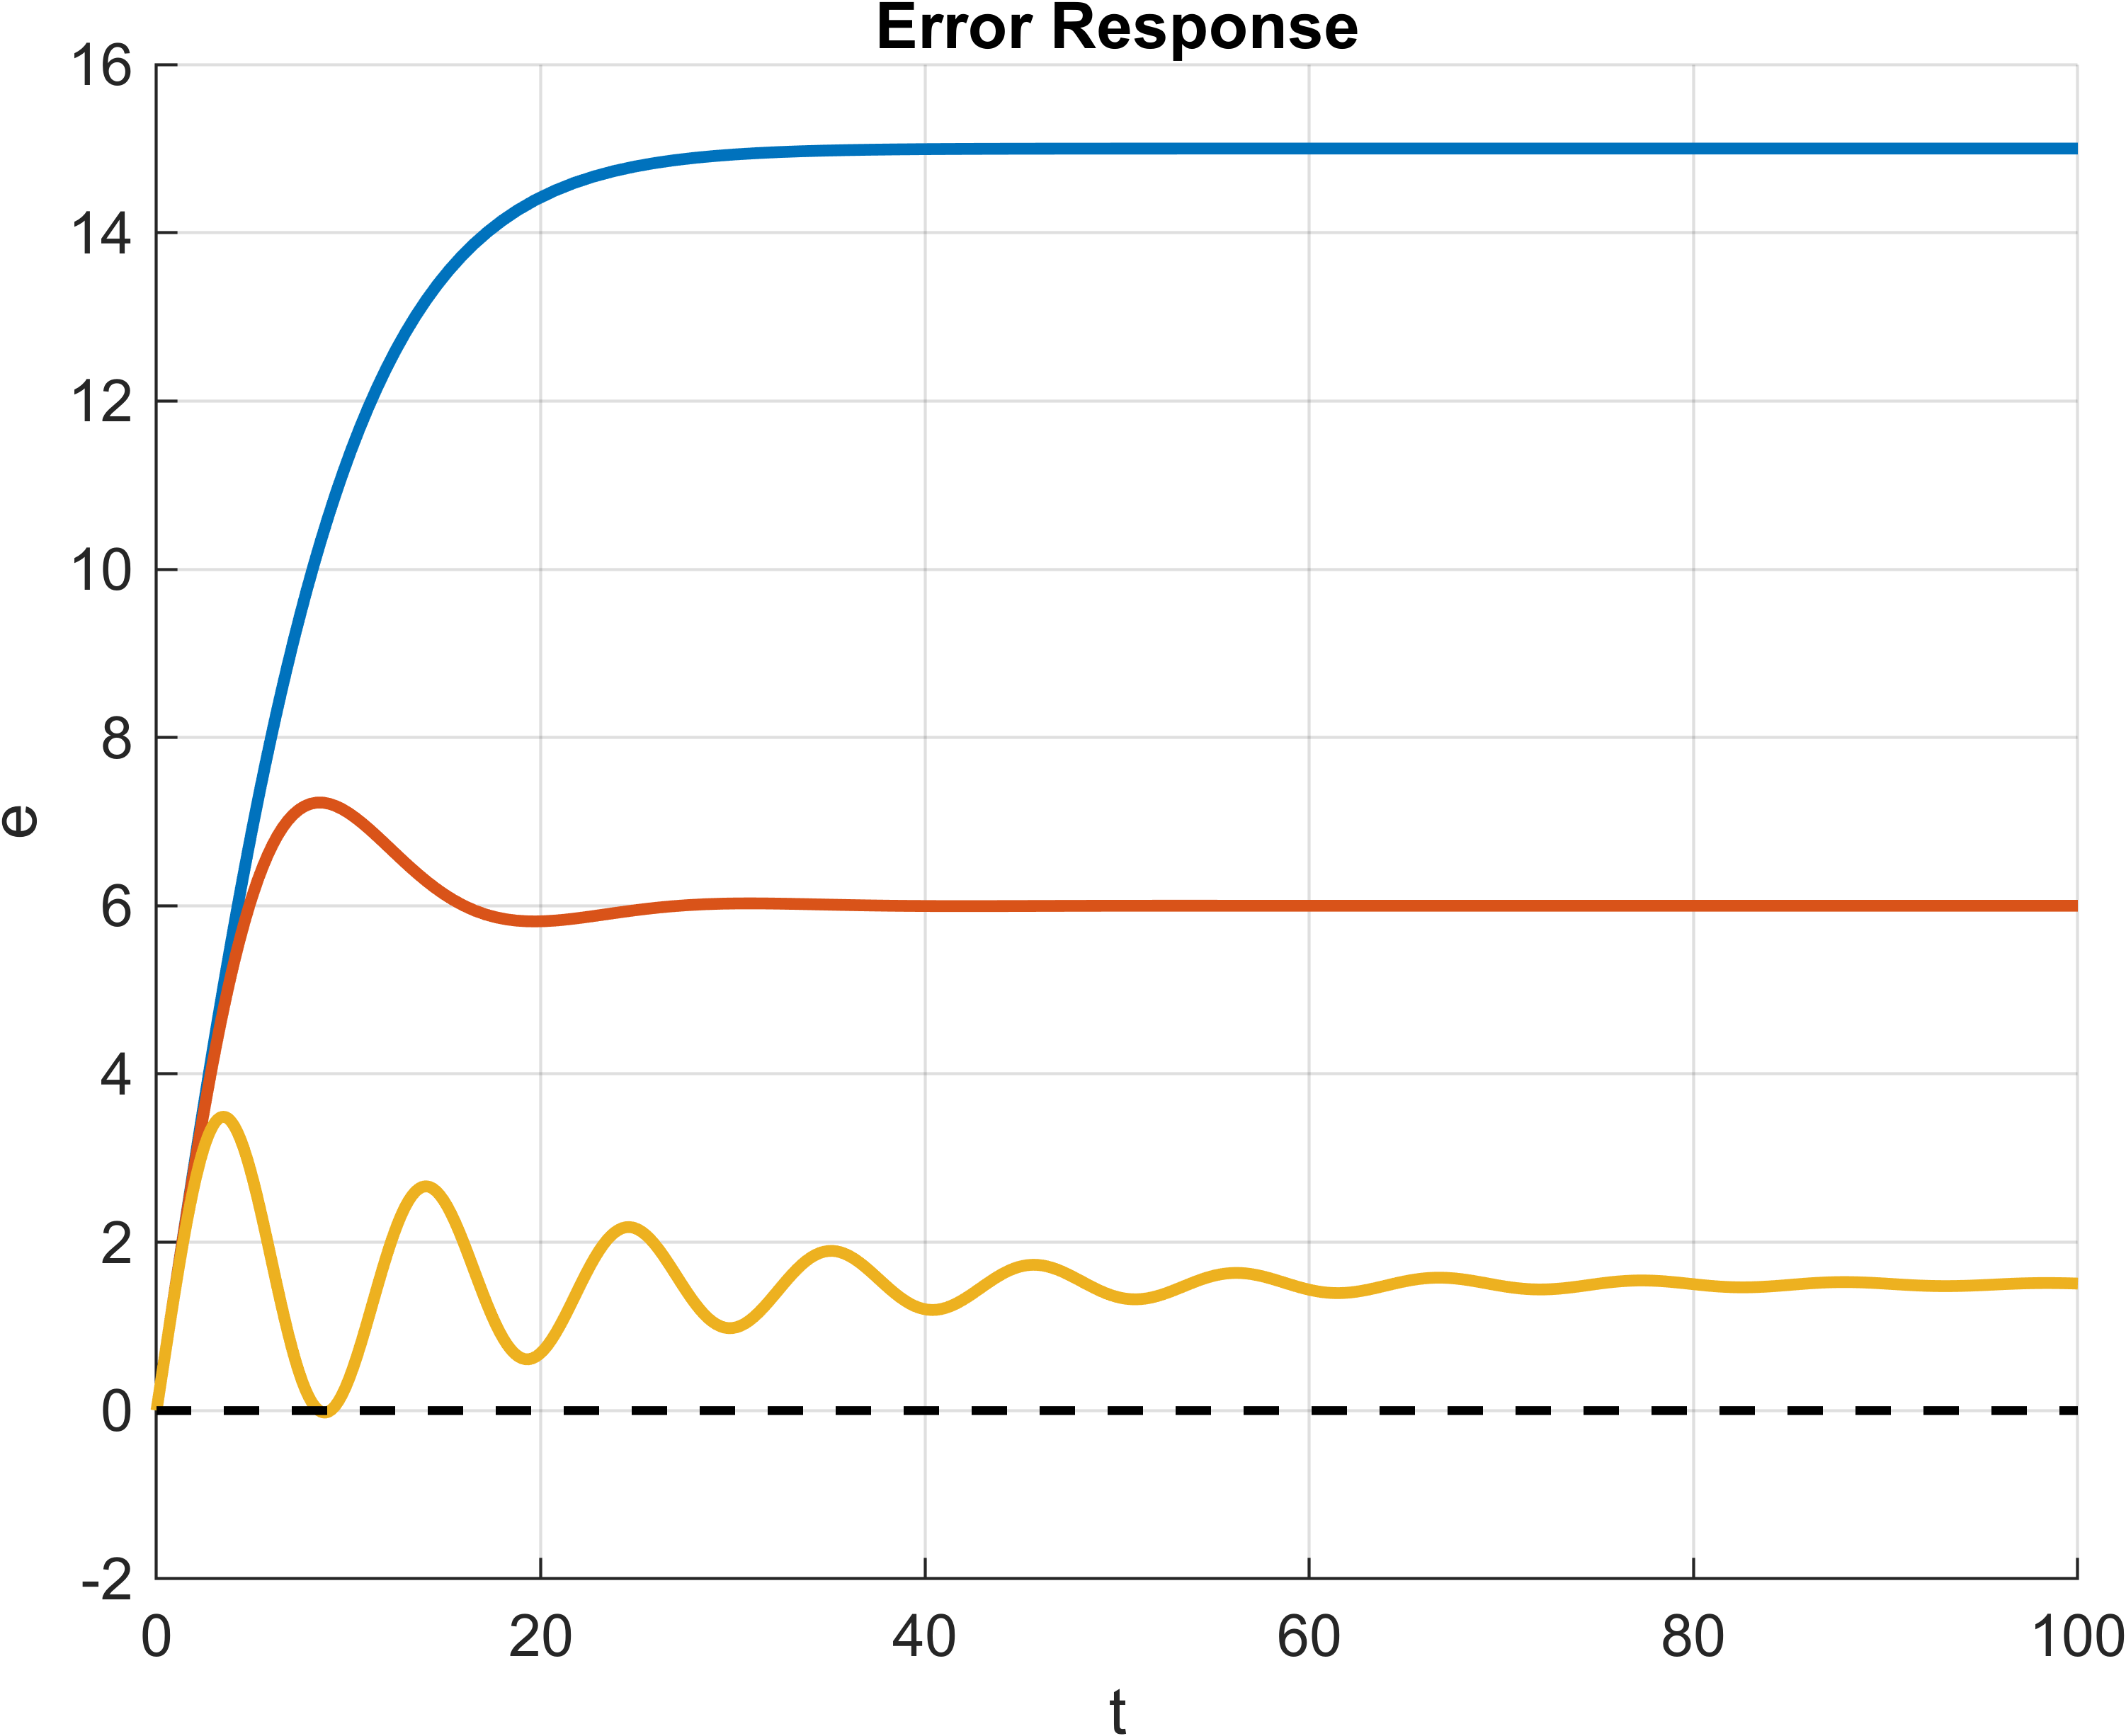
\includegraphics[width=1\textwidth, trim={1cm 0cm 1cm 0cm}]{../images/4_4.png}
    \end{minipage}
    \caption{Графики $y(t)$ и $e(t)$ при $g(t) = 1.5t$}
\end{figure}

Аналитически определим предельное значение ошибки $e$ для каждого значения $k_i$:
\[
W_{g\to e} = \frac{1}{1 + \frac{k_i}{s} W(s)}
= \frac{s}{s + k_i \frac{1}{2s^2 + 3s + 1}}
= \frac{2s^3 + 3s^2 + s}{2s^3 + 3s^2 + s + k_i}
\]
\[
e_{\text{уст}} = \lim_{t \to \infty} e(t)
= \lim_{s \to 0} s E(s)
= \lim_{s \to 0} s W_{g\to e} G(s) =
\]\[
= \lim_{s \to 0} s \frac{2s^3 + 3s^2 + s}{2s^3 + 3s^2 + s + k_i} \frac{1.5}{s^2}
= \frac{1.5}{k_i}
\]
\[
k_i = 0.1: \, e_{\text{уст}} = 15
\]
\[
k_i = 0.25: \, e_{\text{уст}} = 6
\]
\[
k_i = 1: \, e_{\text{уст}} = 1.5
\]

Как видно из графиков и аналитических расчетов, для режима движения с постоянной
скоростью И-регулятор, так как имеет порядком астатизма 1,
обеспечивает постоянную установившуюся ошибку. 
При увеличении коэффициента $k_i$ ошибка уменьшается.
\newpage
\section{Режим движения с постоянным ускорением $g(t) = \frac{at^2}{2}$}
Выполним моделирование:
\begin{figure}[H]
    \centering
    \begin{minipage}{0.45\textwidth}
        \centering
        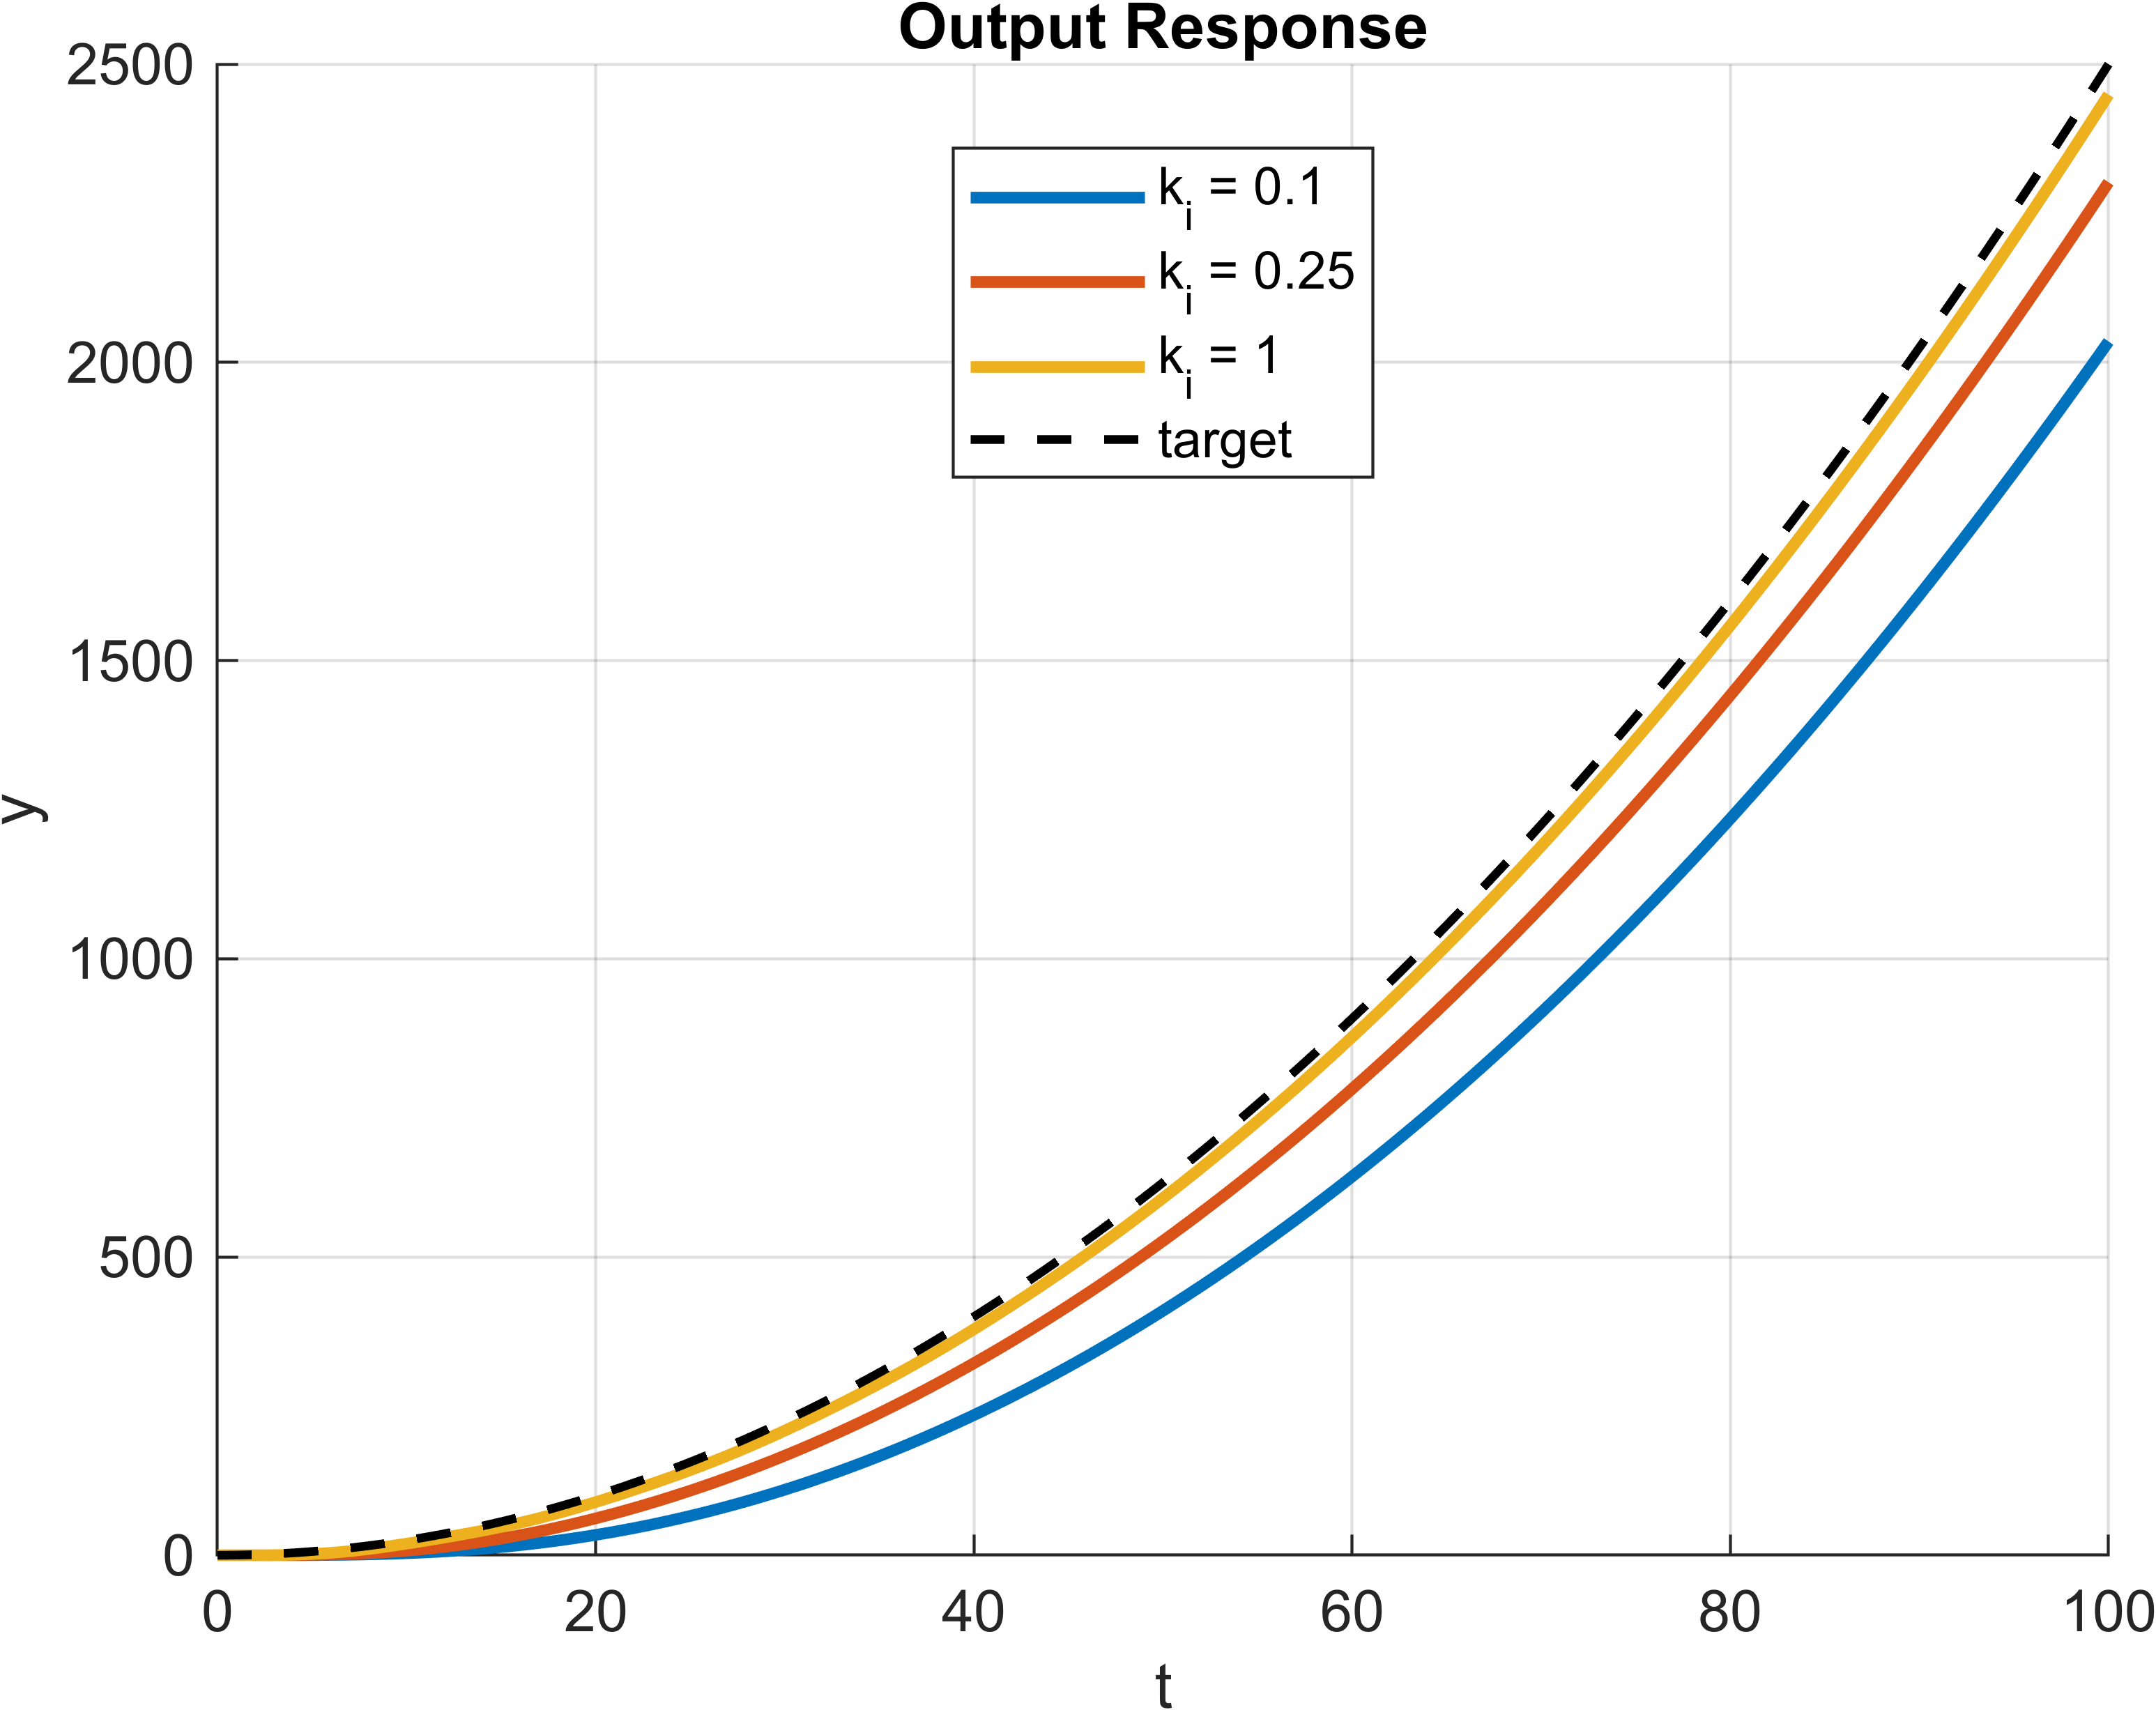
\includegraphics[width=1\textwidth, trim={1cm 0cm 1cm 0cm}]{../images/4_5.png}
    \end{minipage}
    \hfill
    \begin{minipage}{0.45\textwidth}
        \centering
        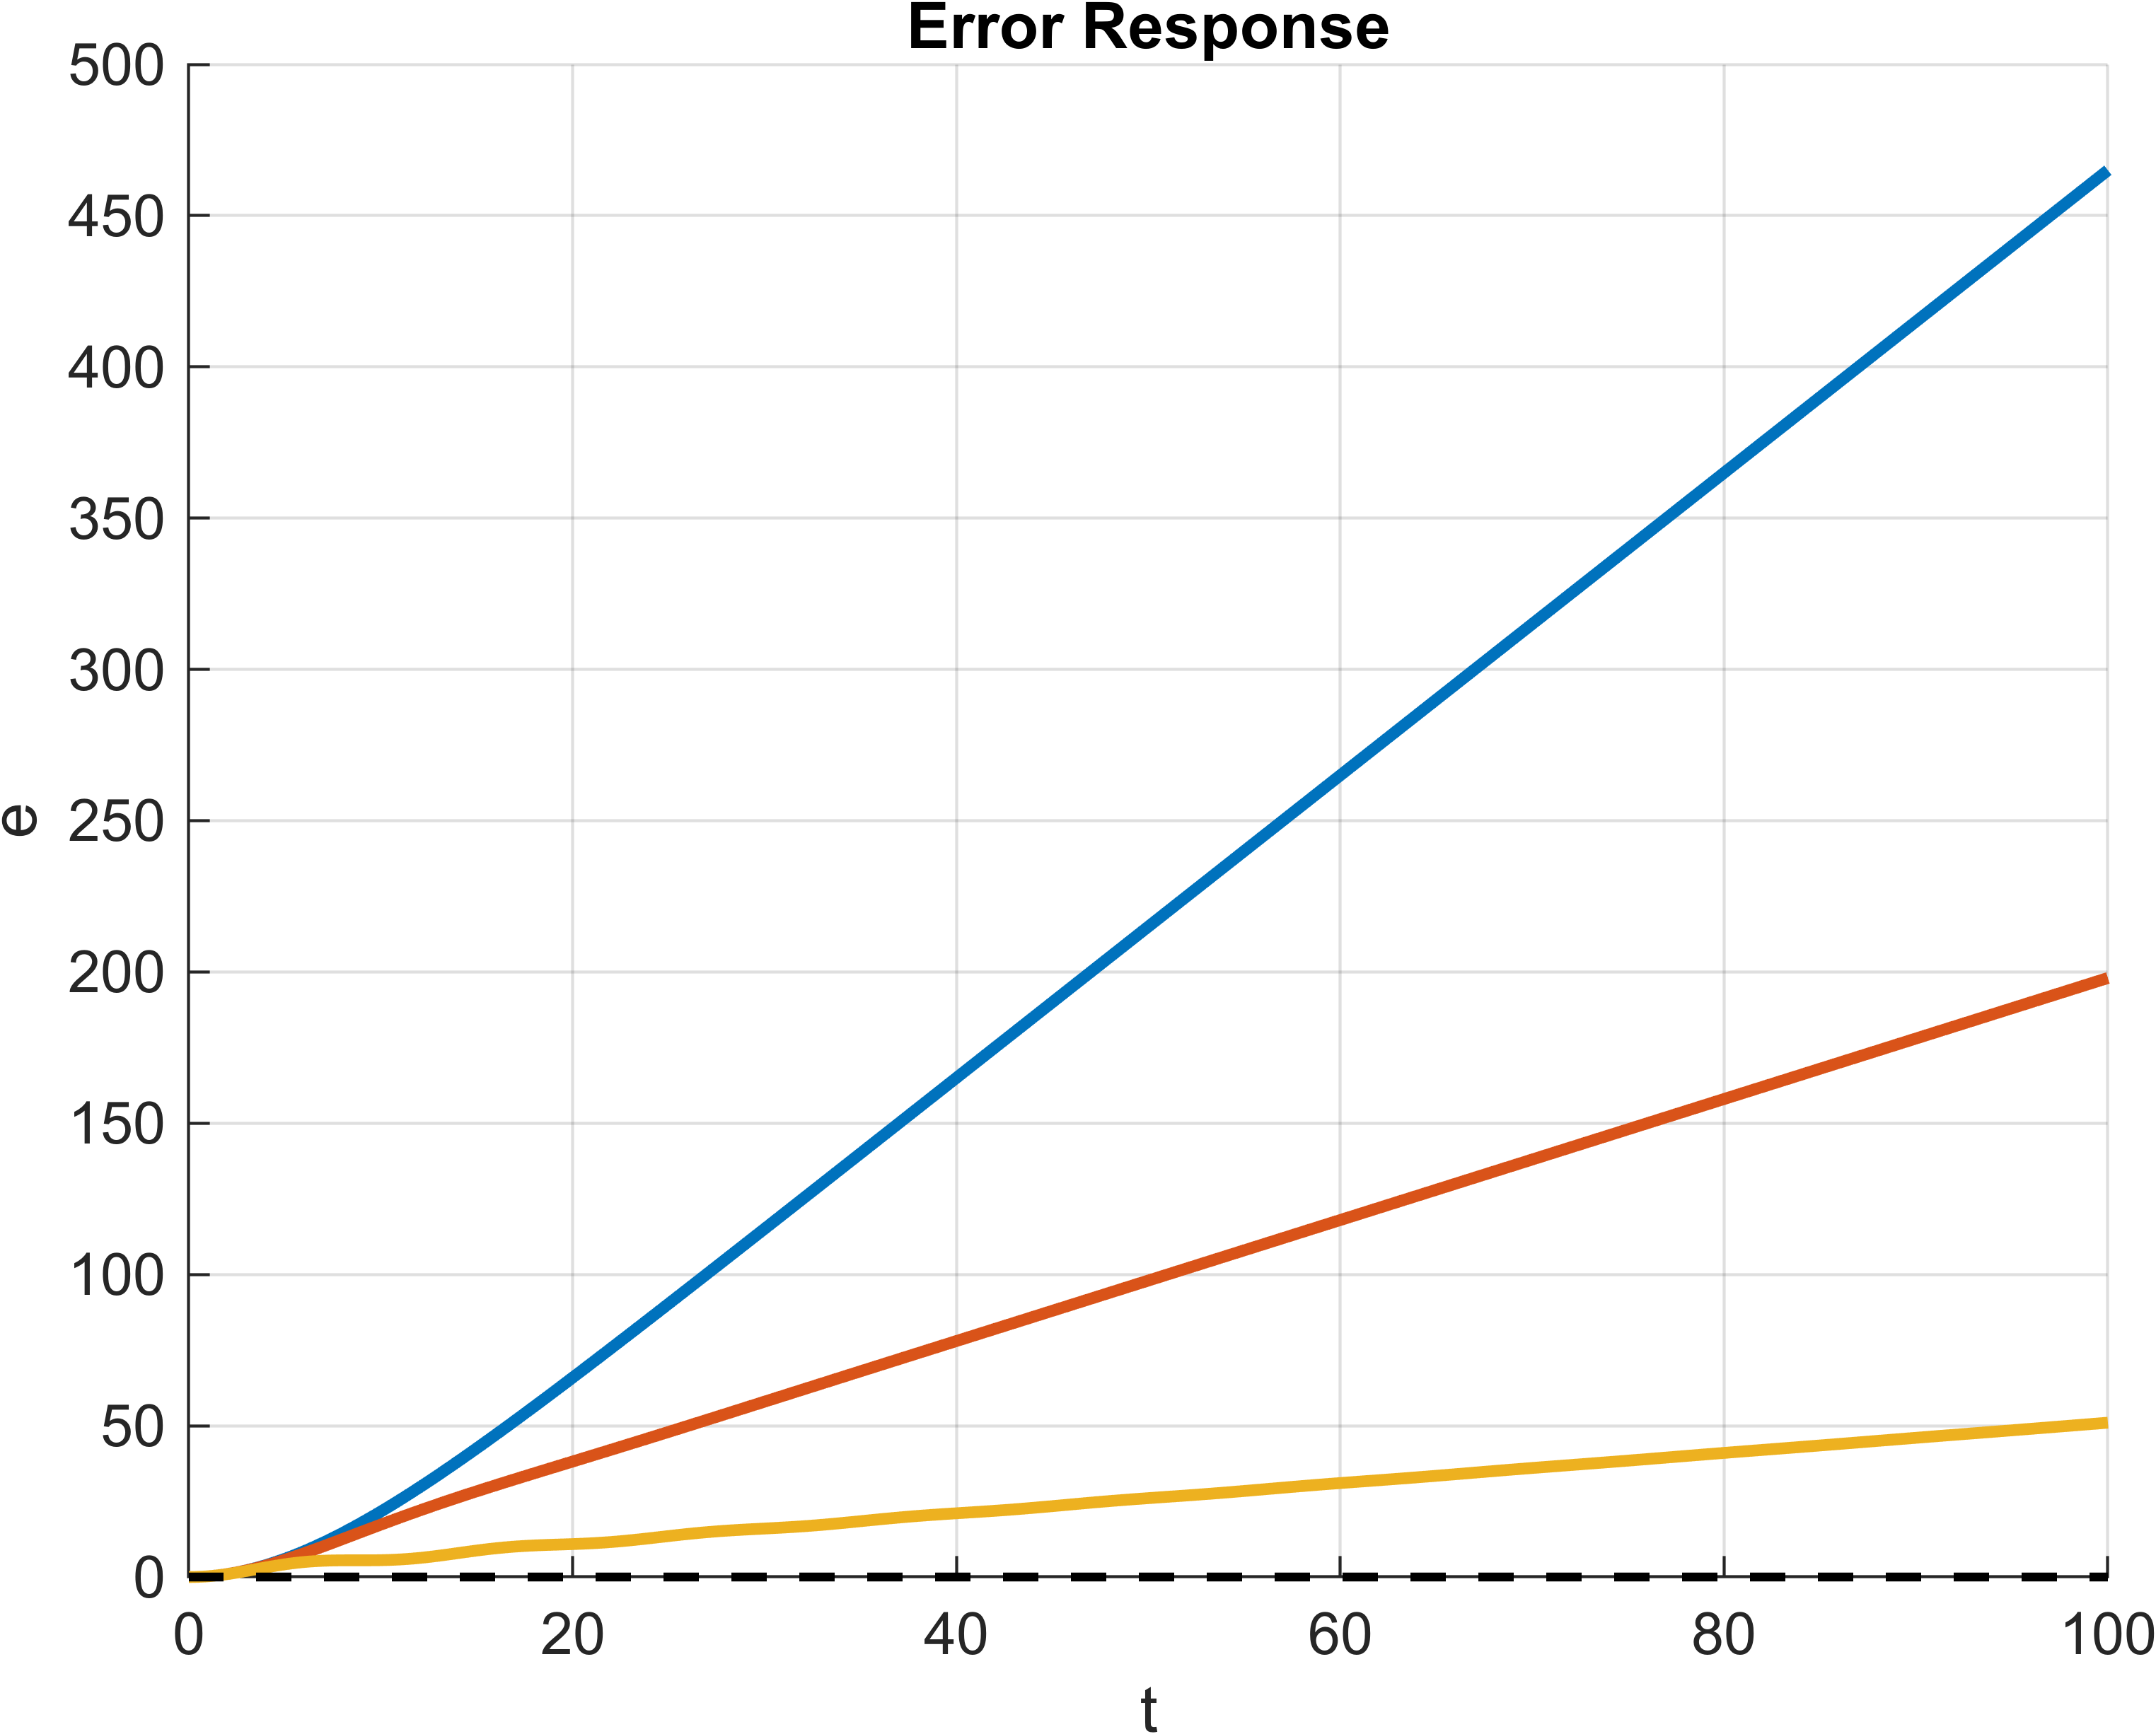
\includegraphics[width=1\textwidth, trim={1cm 0cm 1cm 0cm}]{../images/4_6.png}
    \end{minipage}
    \caption{Графики $y(t)$ и $e(t)$ при $g(t) = 0.25t^2$}
\end{figure}

Так как И-регулятор имеет порядок астатизма 1, то для режима движения с
 постоянным ускорением ошибка бесконечно увеличивается.
 При увеличении коэффициента $k_i$ ошибка увеличивается медленнее.
\endinput